\subsubsection{概要}
むぎまるチームは、ロボットの自己位置推定に
emcl2\_ros2パッケージ\cite{emcl2_ros2}を使用した。
このパッケージでは、LiDARベースのMonte Carlo localization(MCL)と
自己位置推定の破綻を検知してリセット\cite{ueda2004iros}する機能がある。
ロボットの動作計画には、navigation2パッケージ\cite{nav2}を使用した。
使用の際には、パッケージ内の動作計画に関わるソースコードの改造はせず、
起動するノードのパラメータ調整を主に行った。
次項では、これらのソフトウェアとロボットの
システム構成について述べる。

\subsubsection{システム構成}
むぎまるチームのシステム構成についてを図\ref{fig:mugimaru_system}に示す。
Raspberry Piには、ロボットに搭載されたエンコーダとIMUを接続する。
Raspberry Piでは、エンコーダとIMUのセンサデータから
ロボットのオドメトリを計算し、それをROS 2形式の
トピックで配信する処理と、ロボットを速度司令値通りに制御する処理を実行する。
PCには前述のRaspbery Piと3D LiDARを接続する。
PCでは、3D LiDARと受信したオドメトリの情報を用いて、
自己位置推定や動作計画の処理を実行する。
動作計画の結果得られた速度司令値をトピックとして配信する。



\begin{figure}[h]
  \begin{center}
    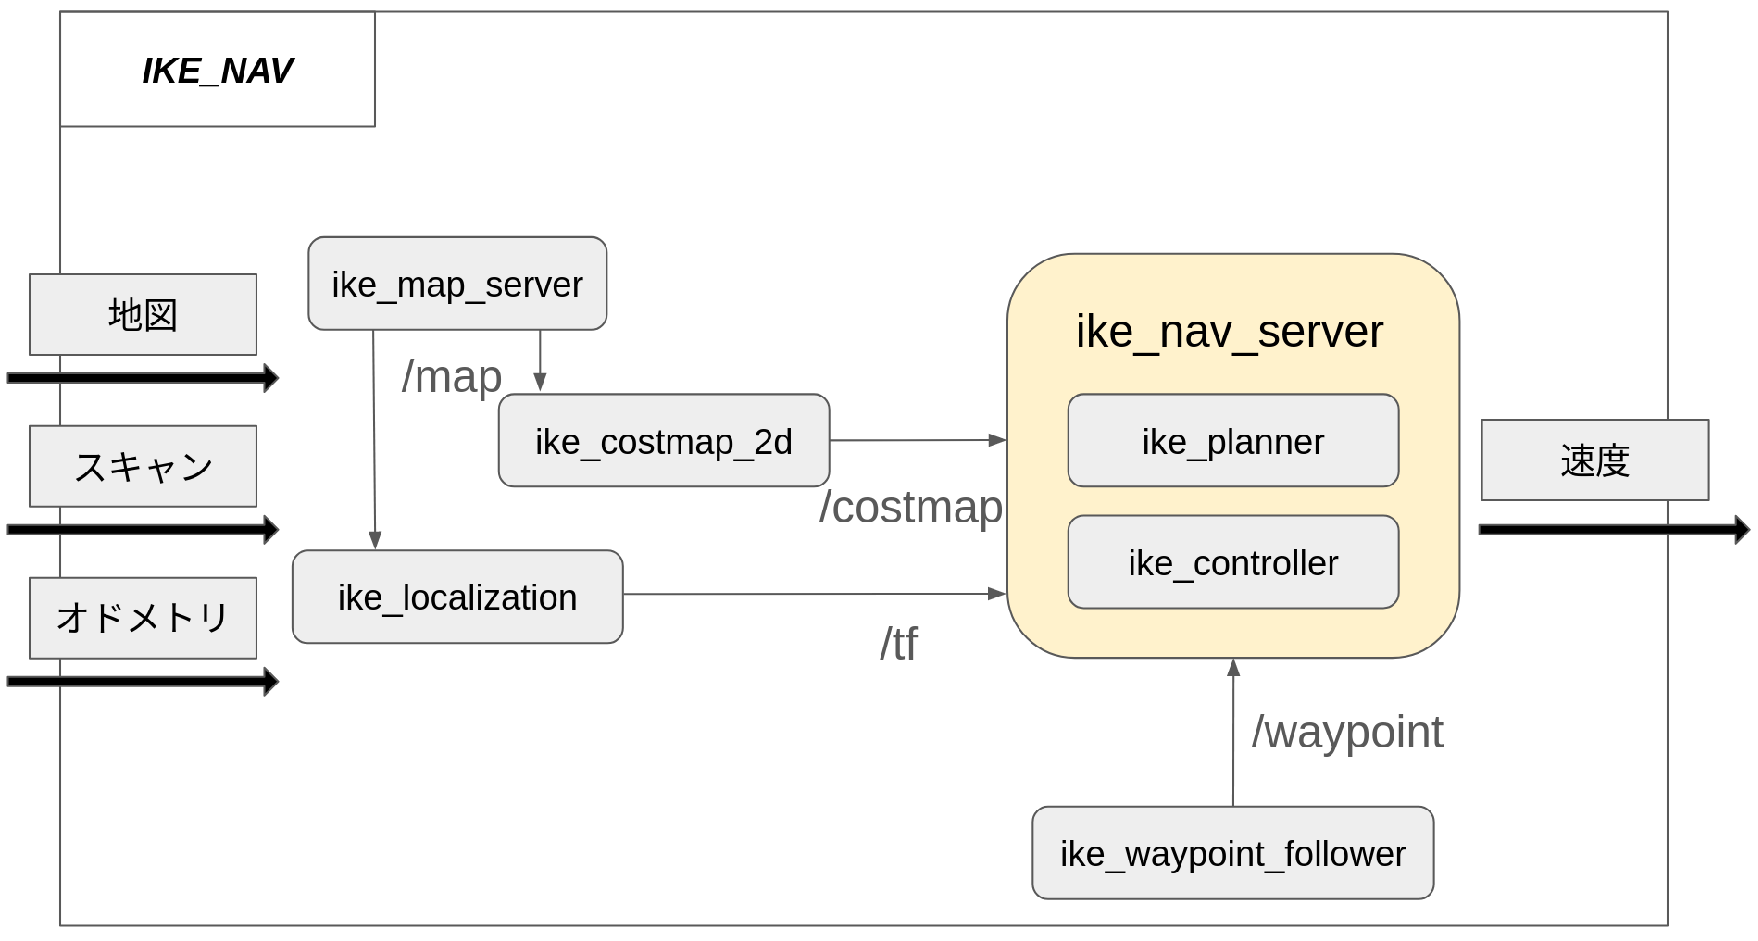
\includegraphics[width=1.0\linewidth]{figs/ike_nav.pdf}
    \caption{ツナチームのシステム構成}
    \label{fig:mugimaru_system}
  \end{center}
\end{figure}

